\documentclass{article} % For LaTeX2e
\usepackage{nips15submit_e,times}
\usepackage{graphicx}
\usepackage{hyperref}
\usepackage{amsmath}
\usepackage{mathtools}
\usepackage{url}
%\documentstyle[nips14submit_09,times,art10]{article} % For LaTeX 2.09


\title{GAN generated and Hand-Drawn Scribble Identification}


\author{
Shubham Malik\\
Department of Computing Science\\
Simon Fraser University\\
\href{mailto:shubhamm@sfu.ca}{\texttt{shubham\textunderscore malik@sfu.ca}} \\
\And
Akash Singh Kunwar \\
Department of Computing Science\\
Simon Fraser University\\
\href{mailto:akunwar@sfu.ca}{\texttt{akash\textunderscore kunwar@sfu.ca}} \\
\AND
Aditi Shrivastava \\
Department of Computing Science\\
Simon Fraser University\\
\href{mailto:ashrivas@sfu.ca}{\texttt{aditi\textunderscore shrivastava@sfu.ca}}
 \\
\And
Rohan Harode \\
Department of Computing Science\\
Simon Fraser University\\
\href{mailto:rharode@sfu.ca}{\texttt{rohan\textunderscore harode@sfu.ca}}
 \\
\\
}

% Using \And between authors leaves it to \LaTeX{} to determine where to break
% the lines. Using \AND forces a linebreak at that point.

\newcommand{\fix}{\marginpar{FIX}}
\newcommand{\new}{\marginpar{NEW}}

\nipsfinalcopy % Uncomment for camera-ready version

\begin{document}


\maketitle

% path for all images
\graphicspath{ {./images/} }

%%%%%%%%%%%%%%%%%%%%%%%%%%%%%%%%%%%%%%%%%%%%%%%%%%%%%%%%
%
%               ABSTRACT
%
%%%%%%%%%%%%%%%%%%%%%%%%%%%%%%%%%%%%%%%%%%%%%%%%%%%%%%%%

\begin{abstract}
\label{abstract}
This paper explores the use of Generative Adversarial Network (GANs) to produce scribbles of different categories. In the project, we also built a multi-class classifier to assign GAN generated or Hand-Drawn scribbles into 7 unique categories. The GAN model generates scribbles with minimal generative loss of 3\% and the classifier guesses the correct category with an accuracy of 87\% and 93\%, implemented on multi-layer perceptron and convolution neural network, respectively, whilst also providing a comparison among other neural network classifiers like random forest and K-nearest neighbors. Experiments were carried out on images from Google’s quick draw [1], which is an open-source dataset of 50 million drawings, and outputs from different models were observed.
\end{abstract}

%%%%%%%%%%%%%%%%%%%%%%%%%%%%%%%%%%%%%%%%%%%%%%%%%%%%%%%%
%
%           SECTION 1 - INTRODUCTION
%
%%%%%%%%%%%%%%%%%%%%%%%%%%%%%%%%%%%%%%%%%%%%%%%%%%%%%%%%


\section{Introduction}
\label{intro}
GANs were introduced by Ian Goodfellow et. al. as “a new framework for estimating generative models via an adversarial process” in a 2014 paper [2]. The network comprises of a generative model that is trained to generate the data to trick the discriminative model, whose job is to classify between ‘real training data’ and ‘fake generated data’. By forcing the network to compete, the generative model is directed to improve its output until the fake generated data is indistinguishable from real training data [2].

In 2016, Google released “Quick Draw”, an experimental game launched to educate people about how AI works which challenges people to draw a given object in 20 seconds. By advancing models on the dataset, we can improve pattern recognition solutions more broadly, which has immediate implications on hand-writing recognition and its application in the areas including Optical Character Recognition (OCR) and Natural Language Processing (NLP).
In this paper, we will explore the use of GAN to generate scribble and then passing the GAN generated image or hand-drawn scribbles to the classifier to categorize it among 7 different categories. The challenge comes with making the model generate highly accurate scribbles, which requires extensive training while minimizing the loss and then training a classifier that predicts the categories accurately while being fast to work in real time.

Similar to this work, Walmart engineer Kirti Pande and Vincent Kuo used the Quick draw dataset [3] to architect a convolutional neural network to tackle sketch classification which predicts the scribbles with an accuracy of 87\% on KNN model. We borrowed the idea of comparing our model with different classifiers like MLP and random forest, but we do not extensively compare with all classifiers due to the limit of time.

%% \subsection{Keywords}

%% \begin{verbatim}
%% GAN
%% Machine Learning
%% Generating
%% classification
%% Convolution Neural Network
%% Multilayer Perceptron
%% Random Forest
%% KNN
%% Flask
%% tensorflow
%% Scribble

%% \end{verbatim}

%%%%%%%%%%%%%%%%%%%%%%%%%%%%%%%%%%%%%%%%%%%%%%%%%%%%%%%%
%
%               SECTION 2 - APPROACH
%
%%%%%%%%%%%%%%%%%%%%%%%%%%%%%%%%%%%%%%%%%%%%%%%%%%%%%%%%

\section{Approach}
\label{approach}
We began to understand the structure of the array that makes up the image. Then we dig deeper to fit some basic classifiers and basic neural network. From there we identified different classifiers we can for our predictions. To determine the success of our classifier's prediction and sketch accuracy of our GAN model, we have used multiple classifiers to predict our scribble(hand-drawn on canvas or gan generated) category. The goal was to classify each scribble with maximum accuracy and avoid miss-classification and efficiently train the GAN model such that it gives minimum loss(GAN loss in section \ref{ganloss}).

\subsection{Dataset}
The dataset, we are using is Quick Draw dataset released by Google[1]. It consist of 28 x 28 grayscale bitmap and converted to a 784 dimensional vector. For GAN model, we are using 75\% of the total number of images of one class to train the GAN model.
To build our classifier, we are using a total of 7 categories, each having 2000 images. We defined our training set to be 80 percent, validation set to 15 percent and test set to 5 percent. Resultantly, we get 11200 images for training set, 2100 images for validation set and 700 images for the test set. The same number of images of every class goes to training and test set, making each category proportionate.


\begin{center}
          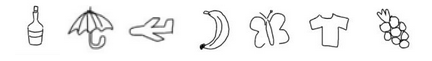
\includegraphics[width=0.9\textwidth]{dataset}\\
      \caption{Sample images of different categories}
\end{center}

\subsection{Training Classifiers}

To get the best model after training, we have used two callback functions: early stopping and model checkpoint. With early stopping callback function, we are monitoring the validation loss and it stops the training once the validation accuracy starts to decrease, whereas, model checkpoint function is used to save the best model. We have added a patience parameter to run for a few more epochs after the validation accuracy decreases. We will pass these callback functions to keras fit function to save the best model, together these callback functions give us the best performing model in a shorter time and thus saving computational resources.

\subsection{Training on GAN}
\bigskip
\begin{center}
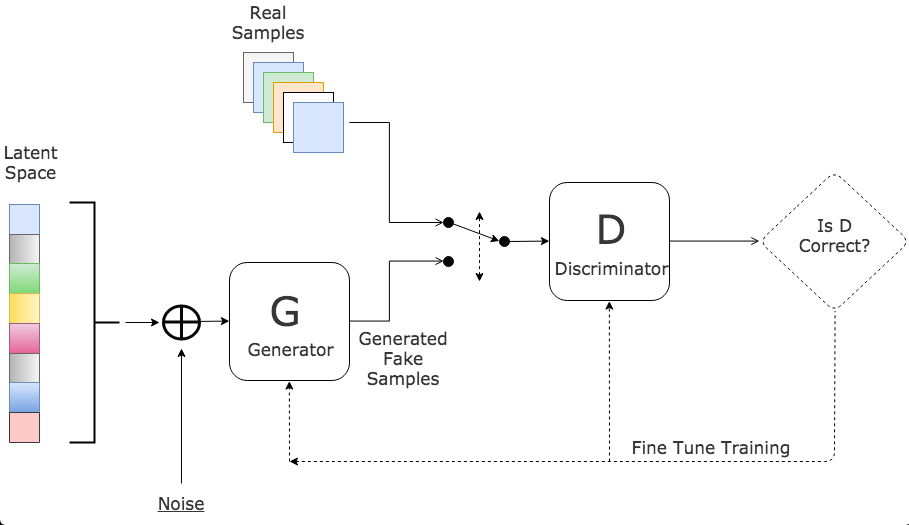
\includegraphics[width=13cm, height=7cm]{gan}
\end{center}
\bigskip
Our model is vanilla GAN with a discriminator and a generator. Generator network creates fake image from noise and tries to fool the discriminator by classifying its output as real. Discriminator network compares real input images with generated (fake) images. The output of the discriminator network penalizes generator with generator loss so that it can modify its generated image to make it more realistic.
 
Initially, we used Batch normalization in the generator network for producing a higher quality of images. However, we didn’t notice any significant effect as it was generating the same quality images for the same batch. We then moved to the gradient penalty method using Adam Optimizers to reduce generator and discriminator losses. 
 
\textbf{Generator:} Inputs are a 100-dimensional Gaussian noise vector \textit{z\textunderscore size}. Outputs a 28x28x1 (\textit{g\textunderscore out}) which is bounded between +1 to -1 since the final layer has \textit{tanh} activation function. No batch normalization is used in hidden layers.
 
\textbf{Discriminator:} Input to discriminator is 28x28 generated image and 28x28x1 real image. The output is a single logit along with final output of network i.e. {d\textunderscore out (real/fake), logits (real/fake)} corresponding to real or generated image. The activation function of Discriminator's final layer is \textit{sigmoid}, making its output restrict between (0,1). Batch normalization is not used after the activation of convolutional layers.
 
\textbf{Hidden Layers:} We used \textit{Leaky ReLU} as activation for hidden layers in the network as they helped the model to perform better and few neurons would die while training once they passes through the Adam optimizer.
The figure below shows the images generated by the GAN model with 3\% maximum loss.
\begin{center}
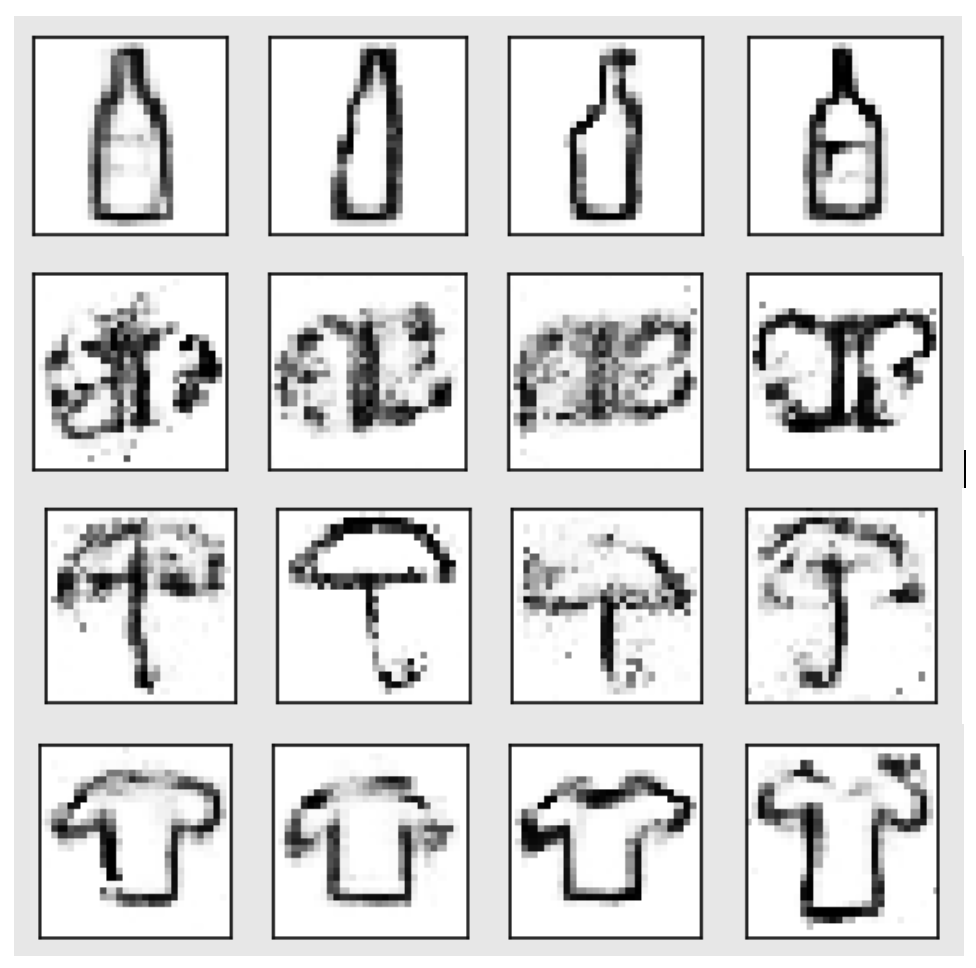
\includegraphics[width=7.5cm, height=8.5cm]{gan_samples}\\
\caption{GAN generated samples}
\end{center}
\subsection{Webapp}
We have created a web application where we put our trained models to test. The application allows users to make predictions of our GAN generated images or their own hand-drawn scribbles. Firstly, the user can select either to draw on Canvas or choose any one of GAN generated images of 7 trained objects. To draw on Canvas, users can select either CNN or MLP model to make predictions whereas for GAN images we have selected CNN as the default model for prediction.
The predict button passes our image data bytes and our dropdown selected values to the flask controller. After preprocessing the image, model's predict method returns the predicted percentage of all the classes and we can see it in the webapp in the form of a pie chart. Figure 1 below shows the prediction using CNN model and hand-drawn image of butterfly, second figure shows the prediction on GAN generated image of butterfly.

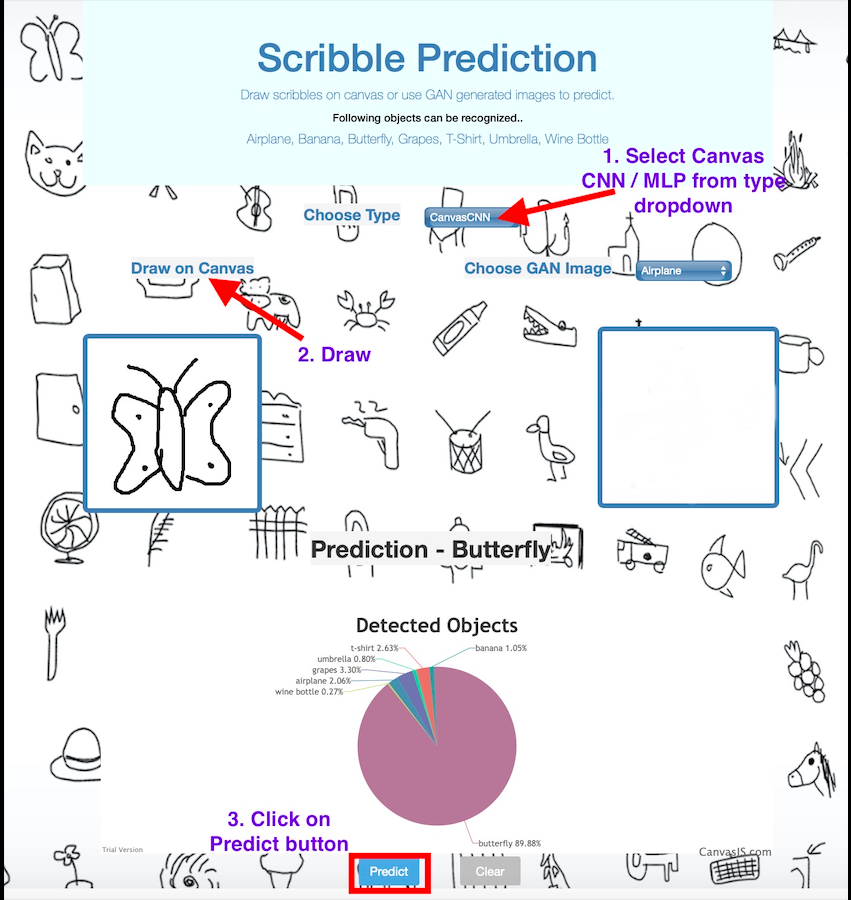
\includegraphics[width=6.9cm, height=7cm]{webapp_cnn}
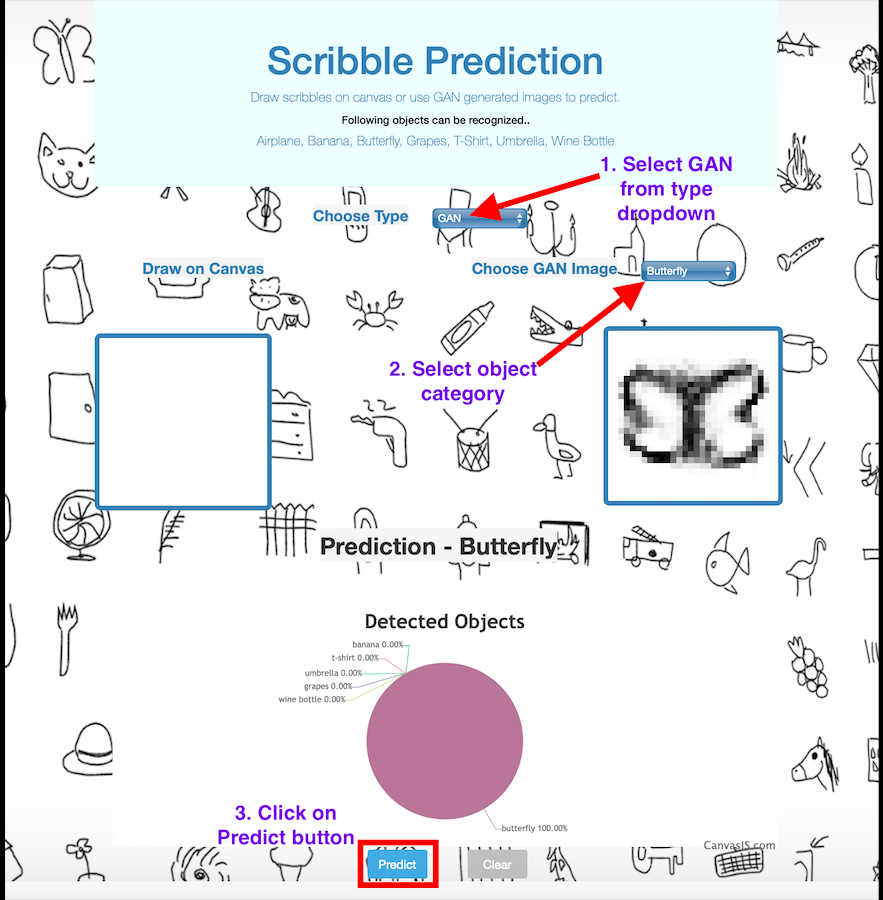
\includegraphics[width=6.9cm, height=7cm]{webapp_gan}

%%%%%%%%%%%%%%%%%%%%%%%%%%%%%%%%%%%%%%%%%%%%%%%%%%%%%%%%
%
%               SECTION 3 - EXPERIMENTS
%
%%%%%%%%%%%%%%%%%%%%%%%%%%%%%%%%%%%%%%%%%%%%%%%%%%%%%%%%



\section{Experiments}
\label{experiments}
\subsection{Random Forest}

The first machine learning technique we used was Random Forest(RF). Considered as the most flexible classification algorithm, Random forest creates decision trees on randomly selected data, gets the prediction from each tree and selects the best solution by the means of voting. 
We used the standard RandomForestClassifier library from scikit-learn and utilized GridSearchCV to cross-validate the model and optimize parameters. We experimented with the number of trees in our random forest and finally settled with n\textunderscore estimators = 100 as our final model.

\subsection{K Nearest Neighbor}
\label{knn}
We then tried the k-Nearest Neighbor (KNN) machine learning algorithm on our dataset. The algorithm assigns an unknown data point to a class by finding the most common class among the k-closest examples.  We used the standard KNeighborsClassifier library from scikit-learn and similar to Random Forest, used the GridSearchCV to cross-validate the model and optimize parameters[4]. Our final model used k = 5.

\subsection{Multilayer Perceptron}
\label{mlp}
Before using the model, we have loaded the dataset with reshape value set to false because the images are needed to be flattened in the case of MLP. We are using model sequential API to create models layer-by-layer. Our input layer dimension is 784 (28 x 28). We are using the activation function \textit{ReLU}. We have also added a Dropout to avoid overfitting. For the final output layer, we have a dimension equal to the number of classes we used in the training. The output layer has a \textit{softmax} activation function.
The disadvantage of using MLP is that the parameters can grow very high and also neglects spatial information as its inputs are flattened vectors. This motivated us to shift to CNN model.

\subsection{CNN - Convolution Neural Network}
\label{cnn}
Convolutional Neural Network model is well known for analyzing visual imagery, the most popular architecture for image classification[6]. Data preprocessing involved normalizing the values for each image sample. This ensures that each feature has a similar range and the gradient doesn’t become uncontrollable during backpropagation. We then added labels to our images followed by one-hot encoding for the labels.

The model architecture is shown in the figure below. For a scribble of size 28 x 28 x 1, we first run the image through two convolutional layers with 32 and 64 filters respectively and a kernel size of 3 x 3, with stride one and \textit{ReLU} activation function. We also add a zero-padding border around the image so that the resulting outputs have the same dimension. The output then goes through a max-pooling layer with a kernel size of 2 x 2. Following this, is a Dropout layer with a rate of 0.25, which helps prevent overfitting. Finally, the tensor was flattened and passed through a fully connected dense layer with the \textit{ReLU} activation function along with a Dropout layer. The output then goes through one last transformation to produce logits of dimension 7 (total categories) with \textit{softmax} activation that assigns probabilities to each class. The model was trained using cross-entropy loss and Adam optimizer.

\begin{center}
          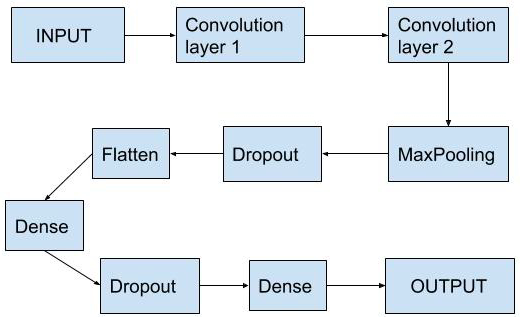
\includegraphics[width=0.6\textwidth]{cnn_arch}\\
%      \caption{Sample images of different categories}
\end{center}


\subsection{GAN Experiments}


\subsubsection{Adjusting Hyperparameters $(learning $ $ rate,$ $ \beta_{1},$ $ \beta_{2})$ for GAN}

The default learning rate for generator and discriminator in the vanilla GAN is 0.002. While training the model, we found the generator loss decreased slowly and converges to a stable value of 2.8 after a considerable number of epochs. The discriminator loss is always low around (0.7 - 0.9). To increase the accuracy of our model and train within an acceptable amount of duration, we decided to decrease the generator and discriminator learning rate to 0.0001. This decreases generator loss to a great extent, and we could record loss values in a range of 1.7 to 2.1. 
 
Default hyperparameters values for both generator and discriminator are \beta_{1}$ = 0, \beta_{2}$ = 0.9[5].
But, after changing the values of hyperparameters to \beta_{1}$ = 0.5,  \beta$_{2}$ = 0.99 we observed a significant decrease in generator loss (2.2 reduced to 0.7) 

\subsubsection{Adjusting number of hidden layers of Generator and Discriminator}
\label{ganloss}
We assessed our model’s accuracy to the number of hidden layers in both the generator and the discriminator network. We discovered that, increase in the number of hidden layers in our model (might be specific to our dataset) results in increasing the generator loss to higher values over epochs while the discriminator loss remains stable at around 0.32. The most optimal design was to include only 1 hidden layer with \textit{ReLU} activation function and pass it to \textit{tanh} and \textit{sigmoid} activation functions for the final output of generator and discriminator respectively. Below are the loss graphs for model with various hidden layers:

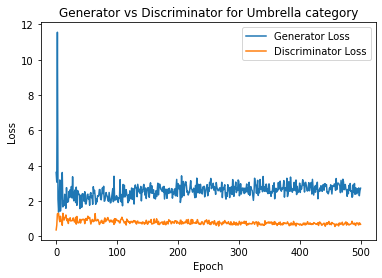
\includegraphics[width=4.3cm, height=5cm]{hiddenlayer1}
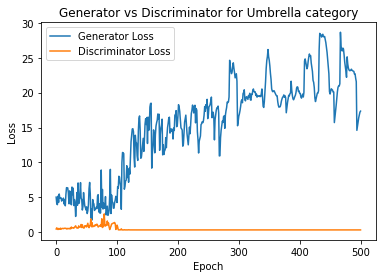
\includegraphics[width=4.3cm, height=5cm]{hiddenlayer2}
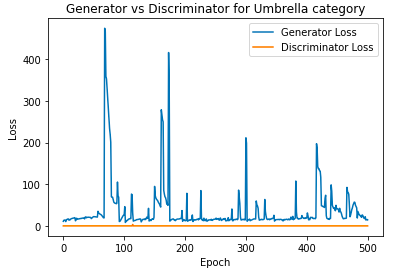
\includegraphics[width=4.6cm, height=5cm]{hiddenlayer3}
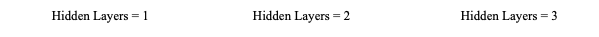
\includegraphics[width=14cm]{cap}

%%%%%%%%%%%%%%%%%%%%%%%%%%%%%%%%%%%%%%%%%%%%%%%%%%%%%%%%
%
%               SECTION 4 - CONCLUSION
%
%%%%%%%%%%%%%%%%%%%%%%%%%%%%%%%%%%%%%%%%%%%%%%%%%%%%%%%%


\section{Conclusion and Future Work}
\smallskip
\label{conclusion}
\subsection{Conclusion}
\smallskip
From the comparison among different classifiers in the table below, it is evident that the best results were obtained using Convolutional Neural Network (CNN)[4] followed by Multilayer Perceptron (MLP). The predicted probabilities for the correctly identified object were quite high in the case of CNN, whereas, in the case of MLP, the predicted probabilities were scattered and there wasn’t any clear majority even for the correctly identified object in some cases. The correctness of images generated using GAN models was exemplary, the CNN classifier was able to predict GAN generated scribbles with more than 98\% accuracy.
\bigskip
\subsection{Future Work}
\smallskip
We approached this problem by dividing our samples to 7 different categories, whereas in reality there are a lot many categories of which scribbles can be drawn. It is sometimes difficult to categorize indistinguishable object drawings, for instance an envelop and door, fence and spreadsheet. The work done by us could be extended in various directions, we will train our model on similar looking scribbles and overcome the model's inability to recognize indistinguishable features and subsequently predicting the sketch more accurately.
Also, due to the high computational requirement of GAN, the model currently operates on 7 objects only. In the future, we plan to expand our code to identify a wider variety of objects. We also plan to implement more complex architectures like VGGNet and AlexNet to obtain a model with even higher accuracy. 
\bigskip
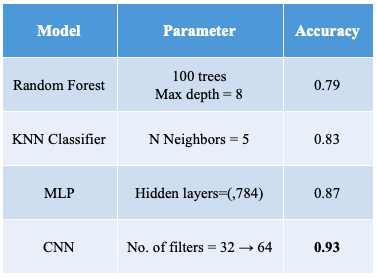
\includegraphics[width=6.5cm, height=5cm]{model_comparison}
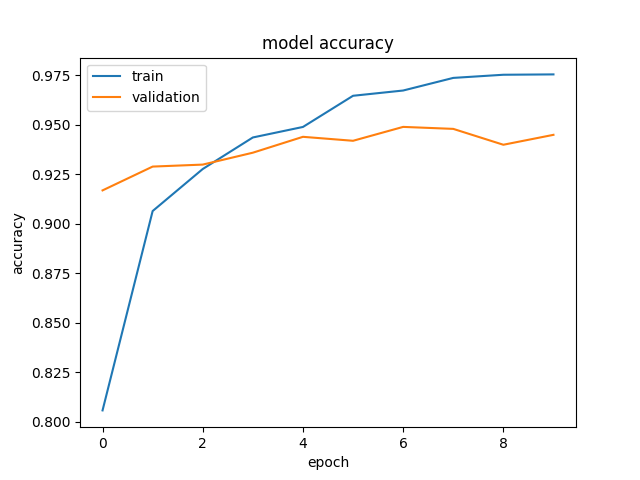
\includegraphics[width=7.3cm, height=5.5cm]{accuracy}
\bigskip

%%%%%%%%%%%%%%%%%%%%%%%%%%%%%%%%%%%%%%%%%%%%%%%%%%%%%%%%
%
%               SECTION 4.5 - CONTRIBUTION
%
%%%%%%%%%%%%%%%%%%%%%%%%%%%%%%%%%%%%%%%%%%%%%%%%%%%%%%%%

\subsection{Contributions}
\bigskip
\begin{center}
 \begin{tabular}{| p{7cm} | p{5cm} |} 
 \hline
 \textbf{Tasks} & \textbf{Members}\\
 \hline\hline
 Topic and Data Set Selection & Aditi, Akash, Rohan, Shubham\\ 
 \hline
 CNN, KNN implementation and research & Aditi, Akash \\
 \hline
 RF implementation and research & Aditi, Rohan\\
 \hline
 MLP implementation and research & Akash, Shubham\\
 \hline
 Training different classifiers & Aditi, Shubham\\
 \hline
 Testing and accuracy improvement & Akash,  Rohan\\
 \hline
 GAN implementation and experiments & Rohan, Shubham\\
 \hline
 Webapp integration & Aditi, Akash, Rohan, Shubham\\
 \hline
 Poster & Aditi, Akash, Rohan, Shubham\\
 \hline
 Report (in Latex) & Aditi, Akash, Rohan, Shubham\\
 \hline
\end{tabular}
\end{center}

\pagebreak
\subsubsection*{References}

\small{
\smallskip

[1]\href{https://github.com/googlecreativelab/quickdraw-dataset#the-raw-moderated-dataset, 2016}{ GoogleCreativeLab, The Quick, Draw! Dataset. https://github.com/googlecreativelab/quickdraw-dataset#the-raw-moderated-dataset, 2016}
\smallskip

[2]\href{https://arxiv.org/abs /1406.2661} { Ian J. Goodfellow, Jean Pouget-Abadie  Jean Pouget-Abadie, Mehdi Mirza, Bing Xu, David Warde-Farley, Sherjil Ozair, Aaron Courville, Yoshua Bengio.:{\it Generative Adversarial nets}}
\smallskip

[3]\href{https://github.com/QuickDraw-sketchRecognition/Sketch_Recognition/}{ Akhilesh Reddy, Vincent Kuo, Kirti Pande, Tiffany Sung, and Helena Shi.:{\it Doodling with Deep Learning!}} 

\smallskip

[4]\href{https://www.ncbi.nlm.nih.gov/pmc/articles/PMC5796274/} { Phan Thanh Noi and Martin Kappas.: {\it Comparison of Random Forest, k-Nearest Neighbor, and Support Vector Machine Classifiers} }

\smallskip
[5]\href{https://arxiv.org/pdf/1710.10196.pdf}{ Karras, T., Aila, T., Laine, S., Lehtinen, J.: {\it Progressive growing of GANs for improved quality, stability, and variation}. In: ICLR (2018)}
\smallskip

[6]\href{https://www.apsl.net/blog/2017/11/20/use-convolutional-neural-network-image-classification/}{ Juan Carlos Gonzalez: Use of Convolutional Neural Network for Image Classification}
\smallskip

[7]\href{https://github.com/diegoalejogm/gans}{ Diego Gomez Mosquera, Google Engineer: {\it Gans: Generative Adversarial Networks} }
}

\end{document}